\documentclass[USenglish]{ifimaster}  %% ... or USenglish or norsk or nynorsk
\usepackage[utf8]{inputenc}           %% ... or latin1
\usepackage[T1]{fontenc,url}
\usepackage[toc,page]{appendix}
\usepackage[backend=biber,style=numeric-comp]{biblatex}
\usepackage[table]{xcolor} %loads also »colortbl«
\usepackage[labelfont=bf]{caption} %labelfont=bf makes figure captions bold
\usepackage{pgfplots}
\usepackage{adjustbox, amssymb, babel, breakcites, float, enumitem, varioref, hyperref, graphicx, array, caption, csquotes, newcent, textcomp, titlesec, duomasterforside, appendix, pdfpages, setspace, listings, subcaption}
% prevents code listing from overflowing

\lstset{
tabsize = 4, %% set tab space width
columns=fullflexible, 
showstringspaces = false, %% prevent space marking in strings, string is defined as the text that is generally printed directly to the console
numbers = left, %% display line numbers on the left
commentstyle = \color{green}, %% set comment color
keywordstyle = \color{blue}, %% set keyword color
stringstyle = \color{red}, %% set string color
rulecolor = \color{black}, %% set frame color to avoid being affected by text color
basicstyle = \small \ttfamily , %% set listing font and size
breaklines = true, %% enable line breaking
numberstyle = \tiny,
}

\makeatother
\onehalfspacing
\urlstyle{sf}

\title{Thesis title}
\subtitle{Thesis subtitle}        

\author{Name}                       

\addbibresource{references.bib} 

\titleformat*{\section}{\LARGE\bfseries}
\titleformat*{\subsection}{\large\bfseries}
\titleformat*{\subsubsection}{\large\bfseries}
\titleformat*{\paragraph}{\large\bfseries}
\titleformat*{\subparagraph}{\large\bfseries}

\begin{document}

\duoforside[dept={Department of Informatics}, program={Programming and System Architecture}, long]                                       
\frontmatter{}

%\chapter*{Preface}

\section*{Abstract}
\input{chapters/0-Abstract}
\newpage

\section*{Acknowledgements}

\newpage

\tableofcontents{}
\listoffigures{}
\listoftables{}
\lstlistoflistings{}

\mainmatter{}

% include chapters here 

\chapter{Introduction}
\label{ch-intro}
\section{Introduction}

Figure \ref{fig:process} shows a typical activity recognition process using machine learning.

\begin{figure}[!ht]
    \centering
    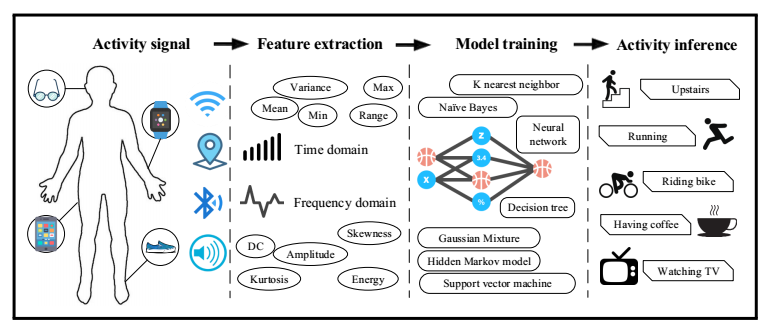
\includegraphics[scale=0.5]{figures/HARML.png}
    \caption{Typical Activity Recognition Process}
    \label{fig:process}
\end{figure}

\appendix
\chapter{Appendix}
\section{Appendix I}


\backmatter{}

\printbibliography

\end{document}